\chapter{Testing} 

\begin{citazione}
Nell'ambito del presente capitolo verranno descritti i risultati ottenuti dalla fase di testing dell'algoritmo implementato. In primo luogo verrà descritto il \emph{Dataset} impiegato per il testing. Successivamente sarà presentato l'ambiente di esecuzione sul quale è stato eseguito l'algoritmo. Infine verranno presentati i tempi di esecuzione di compressione e decompressione con i relativi rapporti di compressione effettuando un confronto tra i risultati ottenuti impiegando diversi algoritmi di \emph{variable length Prefix Code}.
\end{citazione}
\newpage

\section{Dataset}
Dal momento che l'algoritmo implementato lavora solo su testo, il \emph{Dataset} impiegato è costituito da diversi file di testo, di tipologia (racconti, codice sorgente, \dots) e lunghezza variabile. I suddetti file sono reperibili al seguente link: https://github.com/vincenzo-emanuele/Progetto-Compressione-Dati/tree/main/src/TestFiles/Input. 
\section{Ambiente di esecuzione}
Per svolgere la fase di testing dell'algoritmo implementato è stato utilizzato un \emph{MacBook Pro M1 (2020)} avente le seguenti specifiche:
\begin{itemize}
    \item S.O.: MacOS Montrey 12.2.1;
    \item CPU: Chip Apple M1;
    \item RAM: 8 GB;
    \item SSD : 512 GB;
    \item Versione di Python installata: 3.8;
\end{itemize}
\section{Risultati}\label{section:risultati}
La fase di testing condotta ha come scopo quello di verificare la bontà dell'algoritmo in termini computazionali (spazio e tempo) e di appurare che la decompressione vada a buon fine senza perdita di informazione, garantendo, dunque, che l'algoritmo di compressione implementato sia \emph{lossless}. Le tabelle \ref{tab:huffman} e \ref{tab:lzw} indicano, per ogni file del \emph{Dataset}, la sua dimensione non compressa, la sua dimensione a seguito della compressione, il tempo impiegato per la compressione (corrisponde al tempo di esecuzione dello script \emph{compression.py} che implementa la \emph{pipeline} di compressione), il tempo impiegato per la decompressione (corrisponde al tempo di esecuzione dello script \emph{decompression.py} che implementa la \emph{pipeline} di decompressione) e il rapporto di compressione ottenuto. In particolare la prima tabella si riferisce alla \emph{pipeline} di compressione che utilizza \emph{Huffman} come algoritmo di \emph{variable length Prefix Code}, mentre la seconda si riferisce alla \emph{pipeline} che fa uso di \emph{Lempel-Ziv-Welch}. Non è stato effettuato un report riguardante \emph{Arithmetic Coding} in quanto l'implementazione utilizzata risulta essere estremamente inefficiente portando a tempi di esecuzione non ragionevoli (nell'ordine di ore). \\ La \emph{pipeline} di testing è implementata dallo script \emph{testing.py} a cui vanno passati i parametri da linea di comando che indicano il nome del file di input e la chiave segreta da utilizzare.
%Huffman
%\begin{center}
    \begin{table}
    \begin{tabular}{||c c c c c c||} 
     \hline
     Input & Size non compr. & Size compr. & Tempo compr. & Tempo decompr. & \% \\ [0.5ex] 
     \hline\hline
     alice29.txt & 148.467 byte & 76.857 byte & 5.94 s & 0.43 s & 48.23\\ 
     \hline
     asyoulik.txt & 125.179 byte & 69.929 byte & 4.49 s & 0.38 s & 44.14\\
     \hline
     grammar.lsp & 3.721 byte & 2.295 byte & 0.04 s & 0.013 s & 38.33\\
     \hline
     lcet10.txt & 426.754 byte & 202.627 byte & 14.79 s & 1.43 s & 52.52\\
     \hline
     plrabn12.txt & 481.861 byte & 265.036 byte & 16.08 s & 1.75 s & 45.00\\ [1ex] 
     \hline
    \end{tabular} 
    \caption{Risultati ottenuti con Huffman\label{tab:huffman}}
    \end{table}
%LZW
    \begin{table}
    \begin{tabular}{||c c c c c c||}
     \hline
     Input & Size non compr. & Size compr. & Tempo compr. & Tempo decompr. & \% \\ [0.5ex] 
     \hline\hline
     alice29.txt & 148.467 byte & 80.825 byte & 5.55 s & 0.28 s & 45.56\\ 
     \hline
     asyoulik.txt & 125.179 byte & 73.653 byte & 4.20 s & 0.25 s & 41.17\\
     \hline
     grammar.lsp & 3.721 byte & 2.348 byte & 0.05 s & 0.009 s & 36.90\\
     \hline
     lcet10.txt & 426.754 byte & 213.826 byte & 14.14 s & 1.04 s & 49.89\\
     \hline
     plrabn12.txt & 481.861 byte & 281.827 byte & 15.94 s & 1.21 s & 41.51\\ [1ex] 
     \hline
    \end{tabular} 
    \caption{Risultati ottenuti con LZW\label{tab:lzw}}
    \end{table}
%\end{center} 
\begin{figure}[h]
    \centering
    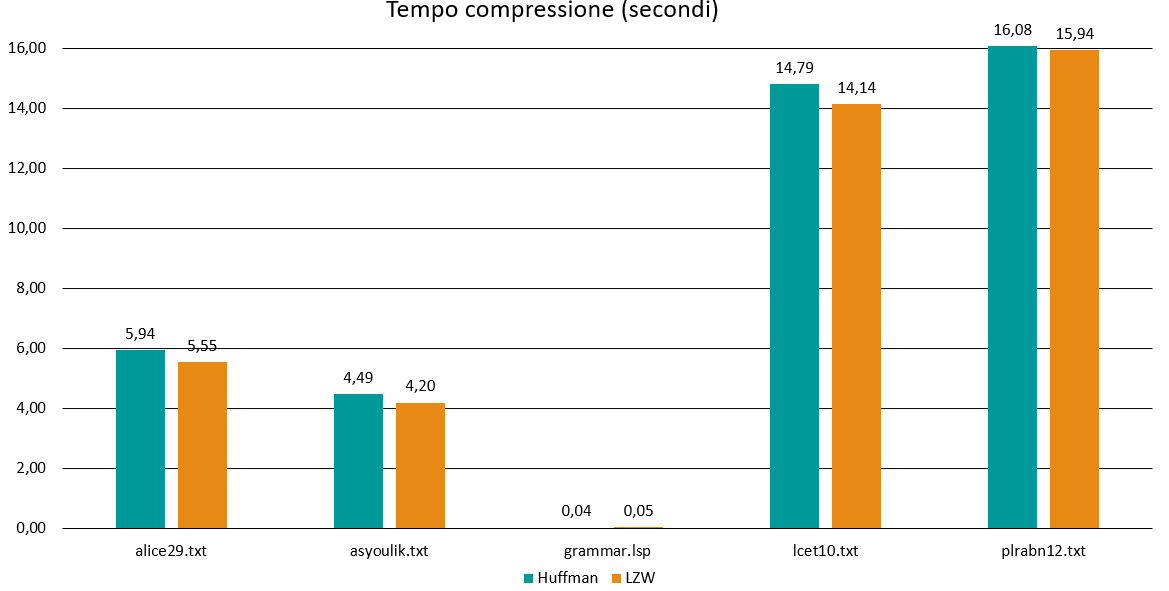
\includegraphics[scale=0.5]{Progetto Compressione Dati/capitoli/images/ist1.png}
\caption{Tempo di compressione}
    \label{fig:ist1}
\end{figure} 
\begin{figure}[h]
    \centering
    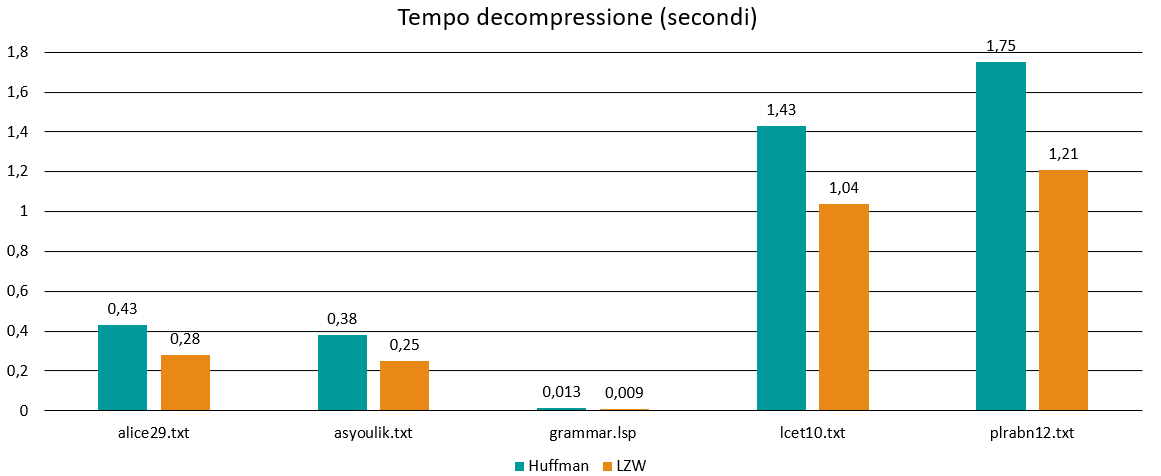
\includegraphics[scale=0.5]{Progetto Compressione Dati/capitoli/images/ist2.png}
\caption{Tempo di decompressione}
    \label{fig:ist2}
\end{figure} 
\begin{figure}[h]
    \centering
    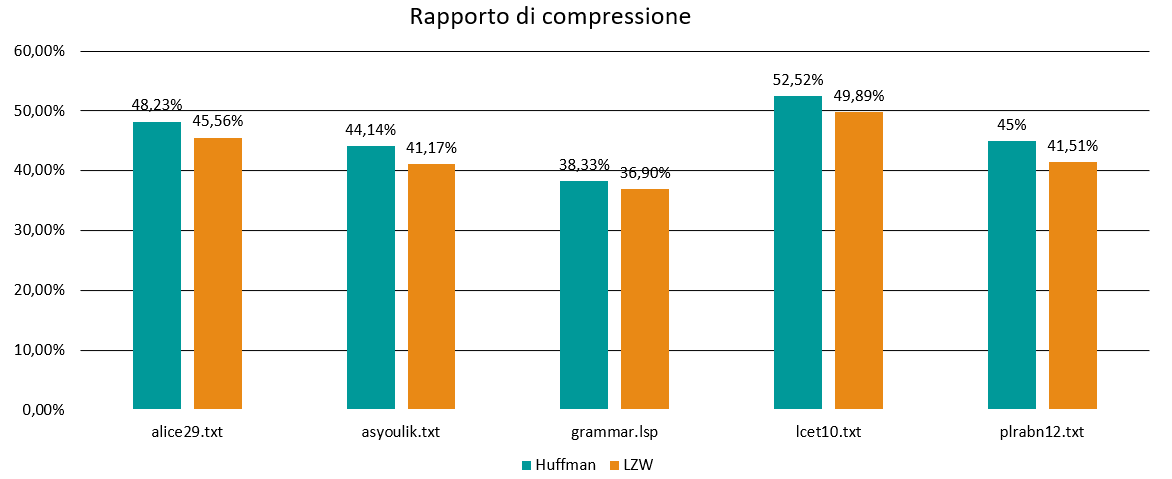
\includegraphics[scale=0.5]{Progetto Compressione Dati/capitoli/images/ist3.png}
\caption{Rapporto di compressione}
    \label{fig:ist3}
\end{figure} 
Come evidenziato dagli istogrammi \ref{fig:ist1} \ref{fig:ist2} e \ref{fig:ist3}, non sono state riscontrate differenze evidenti tra l'utilizzo di \emph{Huffman} e quello di \emph{LZW}. Tendenzialmente \emph{LZW} presenta tempi di esecuzione leggermente più bassi a discapito del rapporto di compressione che nei casi di utilizzo di \emph{Huffman} risulta essere migliore. 
Dopo aver eseguito le fasi di compressione e decompressione, la \emph{pipeline} di testing si assicura che il processo sia avvenuto in maniera \emph{lossless}. Per fare ciò confronta il file di input con l'output della decompressione: se il contenuto di questi due differisce anche solo di un bit, comunicherà a video il fallimento della decompressione. Tale verifica ha restituito esito positivo su ognuno dei file del \emph{Dataset} utilizzato.